\documentclass[a4paper,fleqn]{cas-sc}

\usepackage[numbers,sort&compress]{natbib}
\usepackage{amsmath,amssymb}
\usepackage{booktabs}
\usepackage{graphicx}
\usepackage{multirow}
\usepackage{algorithm}
\usepackage{algorithmic}
\usepackage{float}
\usepackage{setspace}
\hypersetup{hypertexnames=false}

\makeatletter
\pdfstringdefDisableCommands{%
  \def\@corref{}%
  \def\cnotenum{}%
}
\makeatother

\begin{document}
\let\WriteBookmarks\relax
\renewcommand{\topfraction}{0.95}
\renewcommand{\floatpagefraction}{0.75}
\renewcommand{\textfraction}{0.05}
\newcommand{\HighResolutionOutcomeRMSE}{0.227}
\newcommand{\HighResolutionOutcomeTime}{18.3}
\newcommand{\HighResolutionBatchRMSE}{0.228}
\newcommand{\MaxWeightedIdentityRelative}{$6.61\times10^{-6}$}
\newcommand{\MainRegretBaselineMedian}{$8.33\times10^{-16}$}
\newcommand{\MainRegretOffsetMedian}{$1.11\times10^{-15}$}
\newcommand{\MainRegretMaxMedian}{$1.11\times10^{-15}$}
\newcommand{\MainRegretBaselinePninety}{$5.20\times10^{-14}$}
\newcommand{\MainRegretOffsetPninety}{$4.11\times10^{-14}$}
\newcommand{\MainRegretMaxPninetyVariancePercent}{$5.20\times10^{-12}$}
\newcommand{\PriorReductionMin}{1.7}
\newcommand{\PriorReductionMax}{17.4}
\newcommand{\PriorCurrentBaselineReduction}{5.06}
\newcommand{\PriorCurrentBaselineCI}{[2.15, 8.14]}
\newcommand{\PriorCurrentSparseReduction}{8.48}
\newcommand{\PriorCurrentSparseCI}{[5.73, 11.24]}
\newcommand{\MultiStartOptimizerWarnings}{5}


\shorttitle{Reliability Criteria for Sequential Inspection Planning}
\shortauthors{W. Zhang and X. Zhu}
\title[mode=title]{A Parameterization-Invariant Reliability Criterion for Sequential Inspection Planning in Accelerated Life Tests}

\author[1]{Wenhan Zhang}
\author[2]{Xiaojun Zhu}
\cormark[1]
\ead{Xiaojun.Zhu@xjtlu.edu.cn}

\affiliation[1]{organization={School of Mathematics and Physics, Jiangsu University of Technology},
  city={Changzhou}, postcode={213001}, country={China}}
\affiliation[2]{organization={School of Mathematics and Physics, Xi'an Jiaotong-Liverpool University},
  city={Suzhou}, postcode={215123}, country={China}}
\cortext[1]{Corresponding author}

\begin{abstract}
Recursive information trace optimization (RITO) sequentially updates all pending inspection times in an accelerated life test, but its unweighted Fisher-trace criterion assigns different weights to information components under equivalent model parameterizations. This paper embeds a Bayesian reliability criterion within the same rolling inspection framework. The proposed objective minimizes the posterior average log of the locally approximated variance of complementary log-log reliability at use stress and is invariant under invertible linear reparameterization when the likelihood, prior, and target are transformed together. Eight simulation settings and two factorial experiments use 1000 matched replicates each to compare reliability and trace criteria, planning horizons, and inference choices. Reliability-full has accuracy comparable to Trace-full; only sparse-failure and shape-prior-offset settings show paired intervals above zero. When the coded stress is multiplied by 10, median maximum inspection-time changes are 72.58 and 68.48 hours for Trace-full, compared with 0.015 and 0.014 hours for Reliability-full. Common-posterior fixed-pilot checks confirm objective invariance up to numerical precision, whereas rolling experiments retain sensitivity to posterior discretization and optimization. A covariance-weighted trace comparator is also invariant and has comparable accuracy; the reliability criterion instead directly targets the use-stress estimand. When no failure was detected at the common pilot, first-detection time differences exceeded 1 hour in 100\% and 98.7\% of unweighted-trace pairs, compared with none for the two invariant criteria. The results support reliability-oriented planning when consistent decisions across equivalent model parameterizations are required.
\end{abstract}

\begingroup
\def\casprelimstitle{Parameterization-Invariant Sequential Inspection Planning}
\begin{highlights}
\item A Bayesian reliability criterion is embedded in RITO-style inspection planning.
\item The reliability objective is invariant under linear reparameterization.
\item Equivalent stress codings materially alter unweighted trace inspection plans.
\item Accuracy is comparable while rolling numerical sensitivity is explicitly quantified.
\item Invariant weighted trace and reliability criteria are compared directly.
\end{highlights}
\endgroup

\begin{keywords}
Accelerated life testing \sep Interval censoring \sep Sequential inspection \sep Bayesian experimental design \sep Parameterization invariance \sep Reliability estimation
\end{keywords}

\begingroup
\hfuzz=118pt
\maketitle
\endgroup
\onehalfspacing

\section{Introduction}

Accelerated life tests expose products to elevated stress so that failures can be observed within an affordable duration. The fitted model is then used to estimate reliability at normal operating conditions. This extrapolation is sensitive to the experimental plan, especially when samples are small and planning values are uncertain \citep{nelson2009,meeker2021}. Classical designs choose stress levels, sample allocations, and censoring times using local planning values \citep{chernoff1962}. Bayesian designs replace a single value with a distribution over plausible parameters \citep{chalonerverdinelli1995,zhangmeeker2006,hong2015}. Computational methods such as approximate coordinate exchange support the optimization of comparatively complex Bayesian designs \citep{overstallwoods2017}. These developments reduce dependence on an initial guess, but they do not determine how a test should change after observations arrive.

Periodic inspection adds a second design problem. Failure times are known only within inspection intervals, and later inspections can use the counts already observed. Static designs for such readout data show that inspection placement affects efficiency \citep{yangpan2013,hanbai2020,seo2022}, and generalized linear formulations clarify the corresponding information structure \citep{monroe2011}. Sequential methods instead update the design during the experiment. Relevant examples include sequential stress selection \citep{tangliu2010,lee2018}, dual-objective allocation \citep{lu2019}, and batch sequential stress assignment \citep{tung2021}. Approximate Bayesian inference has been used to select material settings \citep{chen2022}, while Bayesian sample allocation addresses one-shot device experiments \citep{kim2026}. Resource-constrained ALT design has also been formulated through deep reinforcement learning \citep{dasilva2026}. These methods address different decision variables and objectives from inspection timing.

RITO is directly relevant to the present work. It optimizes all pending inspection times, implements the earliest optimized inspection, reestimates the parameters, and repeats \citep{zhang2025rito}. It also accommodates multiple stress groups and fixed inspection counts. RITO therefore already supplies the rolling, full-horizon framework that is sometimes associated with nonmyopic design. Its criterion is the trace of Fisher information evaluated at the current parameter estimate. The trace is convenient and computationally attractive, but it sums information components expressed in parameter-specific units. Equivalent model parameterizations can consequently produce different values and different designs.

General nonmyopic design provides several ways to approximate future decisions. Dynamic programming represents them through nested expectations over future observations \citep{bertsekas2017}. Simulation-based ALT design \citep{erkanlisoyer2000,polsonsoyer2017}, batch-informed planning \citep{jiang2020}, and rollout or lookahead optimization \citep{lam2017,yue2020} address the resulting computational burden in different ways. The present full-horizon batch approximation belongs to this broader literature, but its parameterization behavior is examined separately from the choice of approximation.

Reliability-oriented criteria have a long history in optimal design. A scalar target leads to a variance of the form $g^{\mathsf T}I^{-1}g$ rather than a determinant or trace \citep{silvey1980}. ALT studies have used reliability, quantile, and dual objectives in static and sequential settings \citep{panyang2014,hong2015,lu2019}. The present paper does not claim that such criteria are new. It examines their use within RITO-style sequential inspection and asks a narrower question: should an equivalent coding of the stress-life model change the inspection objective?

We answer this question with a Bayesian reliability-variance criterion. The criterion is invariant under invertible linear reparameterization when the likelihood, prior, and reliability target are transformed together. The unweighted Fisher trace used by RITO does not have this property. The rolling implementation is deliberately shared with RITO so that the comparison concerns the criterion rather than the sequential framework. Full-horizon trace and reliability policies are compared with their one-step counterparts, and a factorial experiment separates posterior averaging from criterion choice. The study does not require reliability planning to produce lower RMSE. Its purpose is to establish consistent design objectives while documenting accuracy and computation.

The paper makes two contributions. First, it embeds a Bayesian scalar-target reliability criterion in RITO-style sequential inspection and establishes the invariance of its planning objective under invertible linear reparameterization. Second, it quantifies the practical effects using eight settings, two inference-by-criterion factorial experiments, and equivalent stress codings, all with 1000 matched replicates. A covariance-weighted trace comparator and first-detection outcomes connect the analysis to both invariant alternatives and operational decisions. The results show material trace-plan changes across equivalent codings, invariant reliability objectives under exact transformations, explicit diagnostics of rolling numerical sensitivity, and comparable estimation accuracy.

\section{Model and information for interval observations}

\subsection{Weibull ALT model and reliability target}

Let $x$ denote transformed stress, with $x=0$ at a reference test condition and $x=x_u$ at use. Lifetime $T$ follows a Weibull distribution with scale $\exp(\alpha+\beta x)$ and shape $1/\sigma$. Its cumulative distribution function is
\begin{equation}
F(t;\theta,x)=1-\exp\left[-\exp\left\{\frac{\log t-\alpha-\beta x}{\sigma}\right\}\right],
\label{eq:cdf}
\end{equation}
where $\theta=(\alpha,\beta,\log\sigma)^{\mathsf T}$. Other log-location-scale families can be used by replacing the lifetime distribution and its derivatives.

Let $T_{\max}$ be the latest permissible inspection time. Inspections occur at $0=\tau_0<\tau_1<\cdots<\tau_K\leq T_{\max}$. Let $N_j$ be the failures in $(\tau_{j-1},\tau_j]$, and let $N_{K+1}$ be survivors at the actual final inspection $\tau_K$. These units are right-censored at $\tau_K$; no additional observation is made at $T_{\max}$ unless $\tau_K=T_{\max}$. The cell probabilities are
\begin{equation}
p_j(\theta)=F(\tau_j;\theta,0)-F(\tau_{j-1};\theta,0),\qquad
p_{K+1}(\theta)=1-F(\tau_K;\theta,0).
\end{equation}
Conditional on $\theta$, the counts follow a multinomial distribution. The log likelihood is $\sum_jN_j\log p_j(\theta)$ apart from a constant \citep{sun2006}.

The inferential target is reliability at time $t_0$ under use stress $x_u$. Since $R(t;\theta,x)=1-F(t;\theta,x)=\exp\{-\exp(z)\}$ with $z=(\log t-\alpha-\beta x)/\sigma$, the complementary log-log transformation is
\begin{equation}
h(\theta)=\log\{-\log R(t_0;\theta,x_u)\}
=z_0=\frac{\log t_0-\alpha-\beta x_u}{\sigma}.
\label{eq:target}
\end{equation}
Let $g(\theta)=\partial h(\theta)/\partial\theta$. Its elements are
\begin{equation}
g(\theta)=\left(-\frac{1}{\sigma},-\frac{x_u}{\sigma},-z_0\right)^{\mathsf T}.
\end{equation}

\subsection{Conditional information for remaining units}

Suppose that inspection $k$ has just occurred and $n_k$ units remain at risk. Future information must be conditional on survival to $\tau_k$. For a candidate sequence $\boldsymbol\tau=(\tau_{k+1},\ldots,\tau_{k+h})$, define conditional cell probabilities
\begin{align}
q_1(\theta)&=\frac{F(\tau_{k+1};\theta,0)-F(\tau_k;\theta,0)}{1-F(\tau_k;\theta,0)},\\
q_j(\theta)&=\frac{F(\tau_{k+j};\theta,0)-F(\tau_{k+j-1};\theta,0)}{1-F(\tau_k;\theta,0)},\quad j=2,\ldots,h,\\
q_{h+1}(\theta)&=\frac{1-F(\tau_{k+h};\theta,0)}{1-F(\tau_k;\theta,0)}.
\end{align}
The expected Fisher information from the remaining units is
\begin{equation}
I_k(\boldsymbol\tau;\theta)=n_k\sum_{j=1}^{h+1}
\frac{\dot q_j(\theta)\dot q_j(\theta)^{\mathsf T}}{q_j(\theta)},
\label{eq:information}
\end{equation}
where $\dot q_j$ is the derivative with respect to $\theta$. Writing $z=(\log t-\alpha-\beta x)/\sigma$ and $\phi(z)=\exp\{z-\exp(z)\}$, the required cumulative distribution derivatives are
\begin{equation}
\frac{\partial F}{\partial\alpha}=-\frac{\phi(z)}{\sigma},\qquad
\frac{\partial F}{\partial\beta}=-\frac{x\phi(z)}{\sigma},\qquad
\frac{\partial F}{\partial\log\sigma}=-z\phi(z).
\end{equation}

Independent normal priors are placed on $\alpha$, $\beta$, and $\log\sigma$. Let $P$ be the prior precision and $C_k$ the covariance computed from the grid posterior. Under a locally quadratic approximation to the log posterior, observed information is estimated by $H_k=C_k^{-1}-P$, the difference between posterior and prior precision. This matrix need not be positive definite in small samples, so no spectral truncation is used. Instead, $P+H_k=C_k^{-1}$ is used directly, and the posterior precision remains positive definite. For a reliability target $h$, the approximate posterior variance after a future plan is
\begin{equation}
v(\theta,\boldsymbol\tau)=g(\theta)^{\mathsf T}
\{P+H_k+I_k(\boldsymbol\tau;\theta)\}^{-1}g(\theta).
\label{eq:variance}
\end{equation}
For multiple stress groups inspected at the same times, let $n_{kg}$ be the number at risk in group $g$ and let $q_{jg}$ denote its conditional cell probability. The group matrices are summed explicitly:
\begin{equation}
I_k(\boldsymbol\tau;\theta)=\sum_g n_{kg}\sum_{j=1}^{h+1}
\frac{\dot q_{jg}(\theta)\dot q_{jg}(\theta)^{\mathsf T}}{q_{jg}(\theta)}.
\end{equation}

\section{Design criteria and parameterization}

\subsection{Trace and reliability criteria}

The full-horizon trace criterion maximizes posterior expected information from all remaining inspections:
\begin{equation}
\mathcal T(\boldsymbol\tau)=\frac{1}{M}\sum_{m=1}^{M}
\operatorname{tr}\{I_k(\boldsymbol\tau;\theta_m)\}.
\label{eq:trace}
\end{equation}
A coordinate-weighted trace comparator uses the current grid-posterior covariance $C_k$ and maximizes
\begin{equation}
\mathcal W(\boldsymbol\tau)=\frac{1}{M}\sum_{m=1}^{M}
\operatorname{tr}\{C_k I_k(\boldsymbol\tau;\theta_m)\}.
\label{eq:weightedtrace}
\end{equation}
This comparator standardizes information by current posterior scales while retaining the full planning horizon. The reliability criterion instead minimizes
\begin{equation}
\mathcal V(\boldsymbol\tau)=\frac{1}{M}\sum_{m=1}^{M}
\log v(\theta_m,\boldsymbol\tau).
\label{eq:utility}
\end{equation}
The logarithm limits the influence of posterior draws with extreme variances. All criteria use the same posterior draws, conditional information, time constraints, optimization starts, and final estimator. Trace-1 and Reliability-1 use only the next inspection. Trace-full, Weighted-full, and Reliability-full optimize all remaining inspections, execute the first, and replan after the next interval count is observed. Fixed uses equally spaced inspections. Static optimizes the full sequence after the common pilot but does not replan. Table \ref{tab:policies} summarizes the central policies.

\begin{table}[pos=t]
\centering
\caption{Central policy definitions. All sequential Bayesian policies use the same posterior grid and final estimator.}
\label{tab:policies}
\footnotesize
\begin{tabular}{llll}
\toprule
Policy & Criterion & Horizon & Replanning \\
\midrule
Trace-1 & Fisher trace & Next inspection & At each inspection \\
Reliability-1 & Reliability variance & Next inspection & At each inspection \\
Trace-full & Fisher trace & All remaining inspections & At each inspection \\
Weighted-full & Covariance-weighted trace & All remaining inspections & At each inspection \\
Reliability-full & Reliability variance & All remaining inspections & At each inspection \\
Static & Reliability variance & All remaining inspections & Pilot only \\
Fixed & None & Equally spaced & Never \\
\bottomrule
\end{tabular}
\end{table}

The full-horizon trace policy represents the RITO criterion with posterior averaging. It is not a complete reproduction of RITO. A separate factorial experiment includes a point-estimate, full-horizon trace policy with two common pilot inspections. This comparison is closer to the original parameter updating rule while retaining a common schedule across groups.

The Bayesian formulation incorporates historical information and parameter uncertainty during rolling updates. This is useful with sparse interval counts and in the single-stress settings, where the acceleration coefficient cannot be identified from the current data alone. We do not assume that posterior averaging improves estimation accuracy; the factorial experiment separates this inferential choice from criterion choice. The invariance of the scalar-target criterion is not inherently Bayesian. It relies on transforming the likelihood, information matrix, prior or planning distribution, and reliability target together.

\subsection{Invariance under linear reparameterization}

Consider an invertible linear transformation $\eta=A\theta$. The likelihood and reliability target are unchanged, so
\begin{equation}
I_{\eta}=A^{-\mathsf T}I_{\theta}A^{-1},\qquad
g_{\eta}=A^{-\mathsf T}g_{\theta}.
\label{eq:transform}
\end{equation}
Consequently,
\begin{equation}
g_{\eta}^{\mathsf T}I_{\eta}^{-1}g_{\eta}
=g_{\theta}^{\mathsf T}I_{\theta}^{-1}g_{\theta}.
\label{eq:invariance}
\end{equation}
If the prior and posterior are transformed together, $P$ and $H_k$ transform in the same way as $I_k$. Thus $v$ in \eqref{eq:variance}, and hence $\mathcal V$ in \eqref{eq:utility}, is invariant. In contrast,
\begin{equation}
\operatorname{tr}(I_{\eta})=\operatorname{tr}(A^{-\mathsf T}I_{\theta}A^{-1})
\end{equation}
need not equal $\operatorname{tr}(I_{\theta})$. By contrast, $C_{\eta}=AC_{\theta}A^{\mathsf T}$ and the cyclic property of trace give $\operatorname{tr}(C_{\eta}I_{\eta})=\operatorname{tr}(C_{\theta}I_{\theta})$, so the covariance-weighted comparator is also invariant. For the full planning precision $B_k=C_k^{-1}+I_k$, the same transformation gives $B_{\eta}=A^{-\mathsf T}B_{\theta}A^{-1}$. This does not require $I_k$ to be nonsingular because $C_k^{-1}$ is positive definite. The scalar-target identity is a standard property of optimal design \citep{silvey1980}, not a new optimality theorem. Its consequences for sequential inspection have received less attention.

For example, replacing coded stress $x$ by $x^*=cx$ requires $\beta^*=\beta/c$. The lifetime distribution and reliability target are unchanged, but the information component for acceleration is multiplied by $c^2$. The trace therefore changes the relative weight assigned to acceleration information. The reliability objective retains the same value.

Invariance holds for the design objective, not for every numerical optimizer. Flat directions, multiple local optima, finite posterior grids, and finite-difference optimization can produce different schedules even when their objective values are nearly identical. The numerical study therefore reports schedule distributions and objective checks rather than claiming exact equality of every computed plan.

\subsection{Rolling implementation}

At stage $k$, let $r$ be the number of inspections remaining. The full-horizon policy minimizes $\mathcal V$ over all $r$ future times, while the one-step policy uses $h=1$. The latest permitted time for the $h$th planned inspection is $L=T_{\max}-(r-h)\Delta$, where $\Delta$ is a required minimum gap.

Ordered times are generated through a softmax map. For $j=1,\ldots,h+1$,
\begin{equation}
w_j=\frac{\exp(z_j)}{\sum_{\ell=1}^{h+1}\exp(z_\ell)},\qquad z_j\in[-7,7].
\end{equation}
Each planned interval is $\Delta+(L-\tau_k-h\Delta)w_j$ for $j=1,\ldots,h$. L-BFGS-B uses an equally spaced start and a warm start from the previous remaining plan. The same parameterization is used for trace optimization.

\begin{algorithm}[t]
\caption{Full-horizon sequential inspection with a chosen criterion}
\label{alg:sequential}
\begin{algorithmic}[1]
\REQUIRE Initial interval counts, inspection budget $K$, latest permissible time $T_{\max}$, minimum gap $\Delta$, and posterior sample size $M$.
\ENSURE Inspection sequence and final reliability estimate.
\STATE Conduct the pilot inspection and compute the initial posterior.
\FOR{$k=2,\ldots,K$}
  \STATE Set $r=K-k+1$ and choose planning horizon $h$.
  \STATE Draw $\theta_1,\ldots,\theta_M$ from the current posterior.
  \STATE Optimize \eqref{eq:trace}, \eqref{eq:weightedtrace}, or \eqref{eq:utility} over ordered future times subject to the remaining budget and $\Delta$.
  \STATE Implement only the first optimized inspection time.
  \STATE Record the new interval counts and update the posterior.
\ENDFOR
\RETURN the inspection sequence and posterior reliability estimate.
\end{algorithmic}
\end{algorithm}

The main experiments use one pilot inspection, and the factorial experiment uses two common pilot inspections to identify the three joint parameters. Default optimization uses an equally spaced start and the previous remaining plan as a warm start, with at most 100 iterations per start (120 for the static design). L-BFGS-B uses bounds $[-7,7]$ and `factr` $=10^7$. Optimizer convergence codes are retained, including line-search warnings rather than only fatal fitting failures. Equivalent-coding comparisons use the same physical start and posterior random seed.

Figure \ref{fig:algorithmflow} summarizes the same rolling process. The two criteria share posterior computation and time constraints; their distinction arises when the full remaining plan is evaluated.

\begin{figure}[pos=t]
\centering
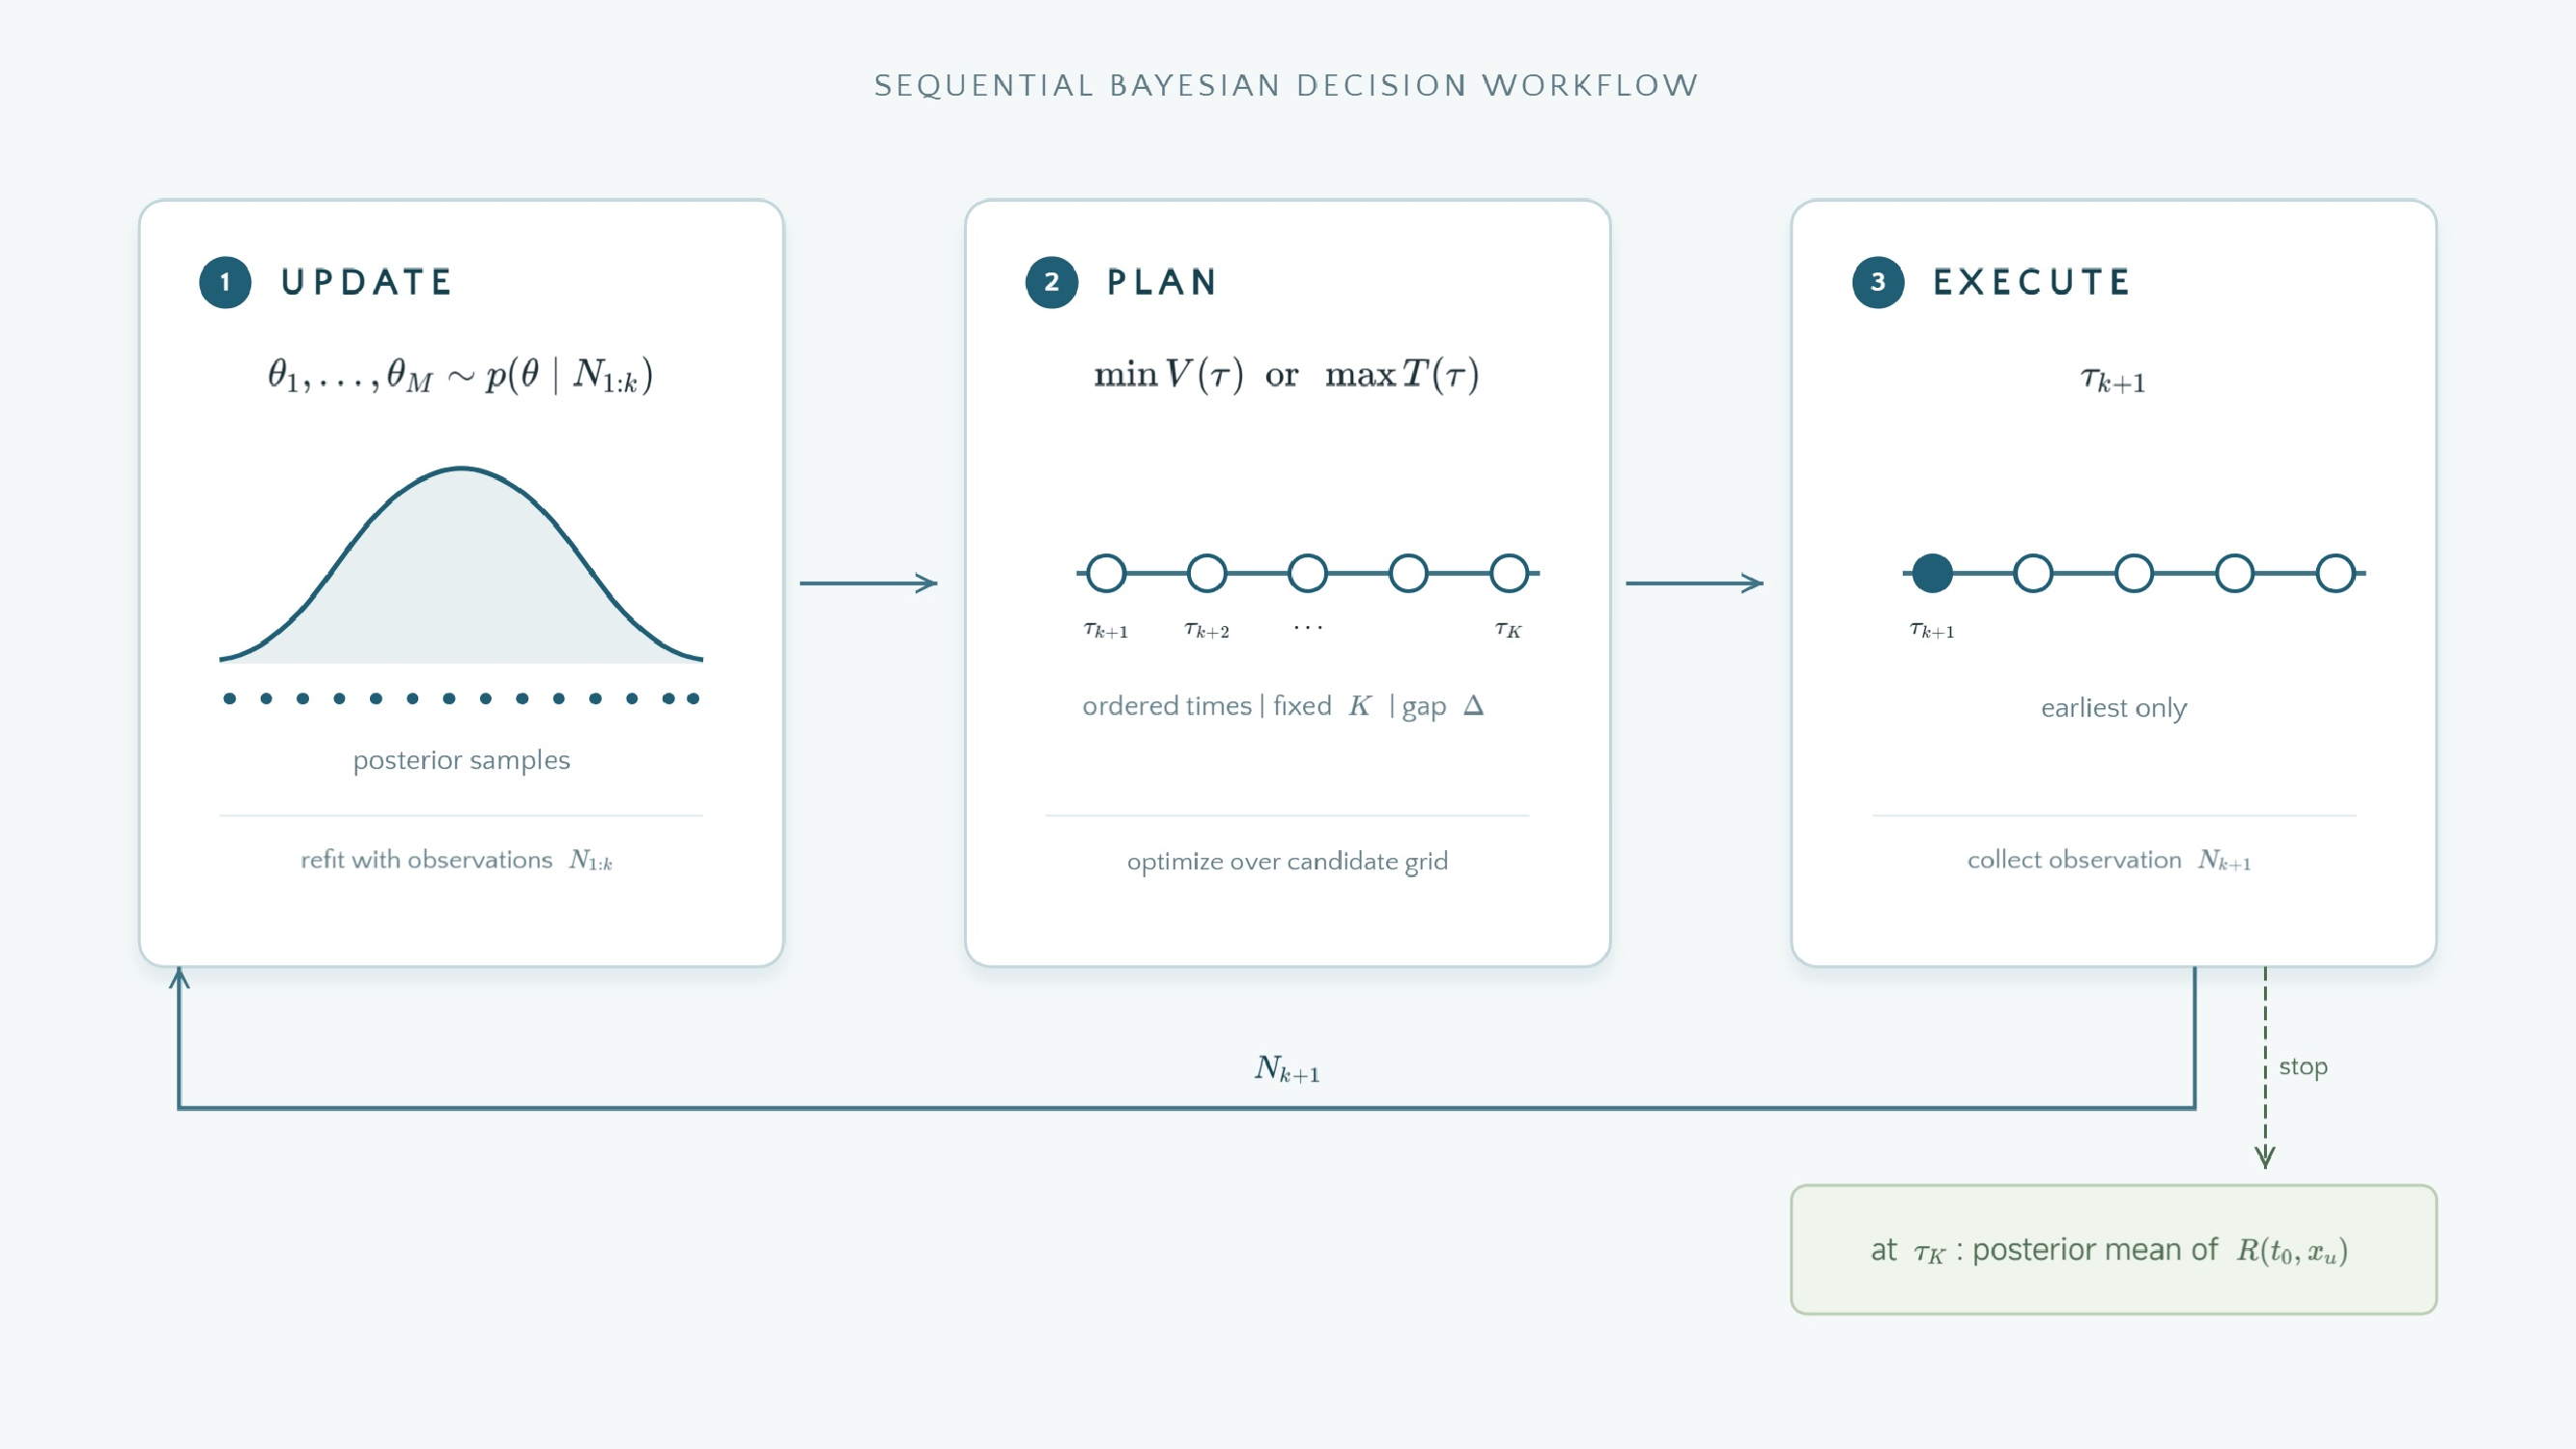
\includegraphics[width=\textwidth]{../output/sequential_bayesian_workflow.pdf}
\caption{Sequential inspection workflow. All remaining times are optimized, only the earliest is executed, and the posterior is updated before the next planning stage.}
\label{fig:algorithmflow}
\end{figure}

\subsection{Posterior computation and checks}

Posterior weights are evaluated from the interval likelihood and prior on a grid over log-location and log-scale parameters. Single-stress models use $41^2=1681$ grid points, and joint models use $21^3=9261$ points. In each direction, the range extends four Laplace standard deviations on either side of the posterior mode, with equally spaced interior points. Grid weights are proportional to the interval likelihood and prior density and are renormalized to sum to one. Laplace optimization constructs only the grid center and scale; it is not the reported posterior approximation. Posterior draws are sampled from the normalized weights, and final estimates are posterior means.

Grid and random-walk Metropolis posteriors were compared on pilot replicate 1 from the baseline, sparse-failure, and location-prior-offset settings, together with the two joint settings. These datasets were selected before inspecting the posterior comparisons. Each MCMC analysis used two chains of 80,000 iterations, with 20,000 warm-up iterations and thinning by 10, giving 12,000 retained target draws. Starting points and proposal covariances came from Laplace fits. Acceptance rates were 0.306 to 0.346 and all target-level $\hat R$ values were below 1.001. Table \ref{tab:posterior} compares posterior means and variances of $h(\theta)$. Detailed grid and optimizer checks are given in Appendix \ref{app:numerical}.

\begin{table}[t]
\centering
\caption{Posterior validation for representative pilot datasets.}
\label{tab:posterior}
% Model version: weibull-cloglog-z0-v2
\begin{tabular}{llrr}
\toprule
Scenario & Method & Posterior mean & Posterior variance \\
\midrule
Baseline & Laplace & -1.805 & 2.520 \\
Baseline & Grid & -1.989 & 0.335 \\
Baseline & MCMC & -1.988 & 0.331 \\
Sparse failures & Laplace & -1.756 & 1.789 \\
Sparse failures & Grid & -1.900 & 0.258 \\
Sparse failures & MCMC & -1.898 & 0.254 \\
Location prior offset & Laplace & -1.521 & 1.764 \\
Location prior offset & Grid & -1.670 & 0.228 \\
Location prior offset & MCMC & -1.668 & 0.222 \\
Two-stress baseline & Laplace & -2.281 & 5.312 \\
Two-stress baseline & Grid3D & -2.634 & 4.775 \\
Two-stress baseline & MCMC & -2.646 & 5.021 \\
Acceleration prior offset & Laplace & -1.571 & 2.718 \\
Acceleration prior offset & Grid3D & -1.828 & 2.011 \\
Acceleration prior offset & MCMC & -1.881 & 2.014 \\
\bottomrule
\end{tabular}

\end{table}

When data come from one elevated stress, $\beta$ is not identifiable from those data alone. Single-stress experiments therefore condition on $\beta$ at its prior mean and update $\alpha$ and $\log\sigma$ on the two-dimensional grid. Both planning and final target draws hold $\beta$ fixed. These are conditional analyses of a supplied acceleration coefficient, not full posterior averaging over its uncertainty. Joint experiments update all three parameters.

\section{Accuracy and computation comparisons}

\subsection{Simulation design}

The main experiments use five inspections, a pilot time of 200, latest permissible time $T_{\max}=1000$, and $\Delta=20$. Survivors are right-censored at the actual fifth inspection, with no additional observation at 1000 h when that inspection occurs earlier. Sample sizes are 30 or 60. The baseline has characteristic test-stress life 1200, $\sigma=0.65$, $\beta=-1$, $x_u=-1$, and $t_0=1000$. Other settings reduce the sample, increase characteristic life to 1800, displace the shape or location prior, use two stress groups, or displace the acceleration coefficient. Joint settings have 30 units at each of $x=0$ and $x=-0.5$ and target $x_u=-1.5$. Table \ref{tab:scenarios} lists the settings.

\begin{table}[t]
\centering
\caption{Simulation settings. The target is $R(1000)$ at the indicated use stress. For two-stress rows, $n=30$ per group, giving 60 units in total.}
\label{tab:scenarios}
\resizebox{\textwidth}{!}{% Model version: weibull-cloglog-z0-v2
\begin{tabular}{lrrrrrrrrrr}
\toprule
Scenario & Groups & $n$ & $\exp(\alpha)$ & $\sigma$ & Prior $\exp(\alpha)$ & Prior $\sigma$ & $\beta$ & Prior $\beta$ & $x_u$ & Target $R$ \\
\midrule
Baseline & 1 & 60 & 1200 & 0.65 & 1200 & 0.65 & -1.0 & -1.0 & -1.0 & 0.850 \\
Small sample & 1 & 30 & 1200 & 0.65 & 1200 & 0.65 & -1.0 & -1.0 & -1.0 & 0.850 \\
Sparse failures & 1 & 60 & 1800 & 0.65 & 1800 & 0.65 & -1.0 & -1.0 & -1.0 & 0.917 \\
Small and sparse & 1 & 30 & 1800 & 0.65 & 1800 & 0.65 & -1.0 & -1.0 & -1.0 & 0.917 \\
Shape prior offset & 1 & 60 & 1200 & 0.50 & 1200 & 0.85 & -1.0 & -1.0 & -1.0 & 0.910 \\
Location prior offset & 1 & 60 & 1200 & 0.65 & 1600 & 0.65 & -1.0 & -1.0 & -1.0 & 0.850 \\
Two-stress baseline & 2 & 30 & 1200 & 0.65 & 1200 & 0.65 & -1.0 & -1.0 & -1.5 & 0.928 \\
Acceleration prior offset & 2 & 30 & 1200 & 0.65 & 1200 & 0.65 & -1.3 & -1.0 & -1.5 & 0.963 \\
\bottomrule
\end{tabular}
}
\end{table}

Every scenario contains 1000 replicates. Failure times and the underlying random uniforms are generated once per replicate and shared by all policies. Posterior sampling uses the same policy seed across criteria, so candidate posterior draws are paired as well as the physical data. Batch policies use 16 posterior draws. Let $e_b=\hat h_b-h_b$ and $\overline{e^2}=B^{-1}\sum_{b=1}^B e_b^2$. For policies $a$ and $b$, $\mathrm{RMSE}=\sqrt{\overline{e^2}}$ and the reported reduction is $100(1-\mathrm{RMSE}_a/\mathrm{RMSE}_b)$. Paired 95\% intervals resample replicate indices jointly 5000 times within each scenario. The influence-function delta method gives $\widehat{\mathrm{SE}}(\mathrm{RMSE})=\operatorname{sd}(\{e_b^2\}_{b=1}^B)/(2\sqrt{B\,\overline{e^2}})$, without a normal-error approximation. All computations use R 4.6.2 and fixed seeds.

Timing covers only the planning optimizer, not posterior grid construction, likelihood fitting, or random-number generation. Independent scenarios were run as separate Rscript processes on an Intel Core Ultra 7 265K computer with 31.37 GB RAM. These times are implementation-specific and are used only for relative comparison.

\subsection{Criterion and horizon}

Table \ref{tab:criterion} compares one-step and full-horizon criteria. Reliability-full has lower RMSE than Reliability-1 in all six single-stress settings, but this comparison does not represent RITO. Against Trace-full, reductions are 0.33\%, -0.25\%, 2.33\%, -2.20\%, 2.12\%, and 0.47\% in the six single-stress settings. Only sparse failures and shape-prior offset have paired intervals above zero, with reductions of 2.33\% [0.37, 4.29] and 2.12\% [0.48, 3.82]. The two joint reductions are -0.31\% and -0.18\%, with intervals covering zero. Reliability-full is therefore comparable to Trace-full in accuracy, not generally better.

\begin{table}[t]
\centering
\caption{RMSE over 1000 matched replicates. Reduction compares Reliability-full with Trace-full.}
\label{tab:criterion}
\resizebox{\textwidth}{!}{% Model version: weibull-cloglog-z0-v2
\begin{tabular}{lrrrrrr}
\toprule
Scenario & Trace-1 & Reliability-1 & Trace-full & Reliability-full & Reduction (\%) & 95\% CI \\
\midrule
Baseline & 0.338 & 0.295 & 0.281 & 0.281 & 0.33 & [-1.66, 2.17] \\
Small sample & 0.454 & 0.420 & 0.396 & 0.397 & -0.25 & [-2.40, 1.76] \\
Sparse failures & 0.433 & 0.406 & 0.381 & 0.372 & 2.33 & [0.37, 4.29] \\
Small and sparse & 0.533 & 0.505 & 0.483 & 0.494 & -2.20 & [-4.65, 0.07] \\
Shape prior offset & 0.381 & 0.363 & 0.344 & 0.337 & 2.12 & [0.48, 3.82] \\
Location prior offset & 0.342 & 0.300 & 0.288 & 0.286 & 0.47 & [-1.32, 2.17] \\
Two-stress baseline & 0.842 & 0.841 & 0.825 & 0.828 & -0.31 & [-0.74, 0.12] \\
Acceleration prior offset & 0.875 & 0.874 & 0.854 & 0.856 & -0.18 & [-0.55, 0.18] \\
\bottomrule
\end{tabular}
}
\end{table}

Figure \ref{fig:rmse} displays the same comparisons. Full-horizon planning is beneficial relative to one-step planning in several settings, but the choice between full-horizon criteria has little effect on RMSE.

\begin{figure}[pos=p]
\centering
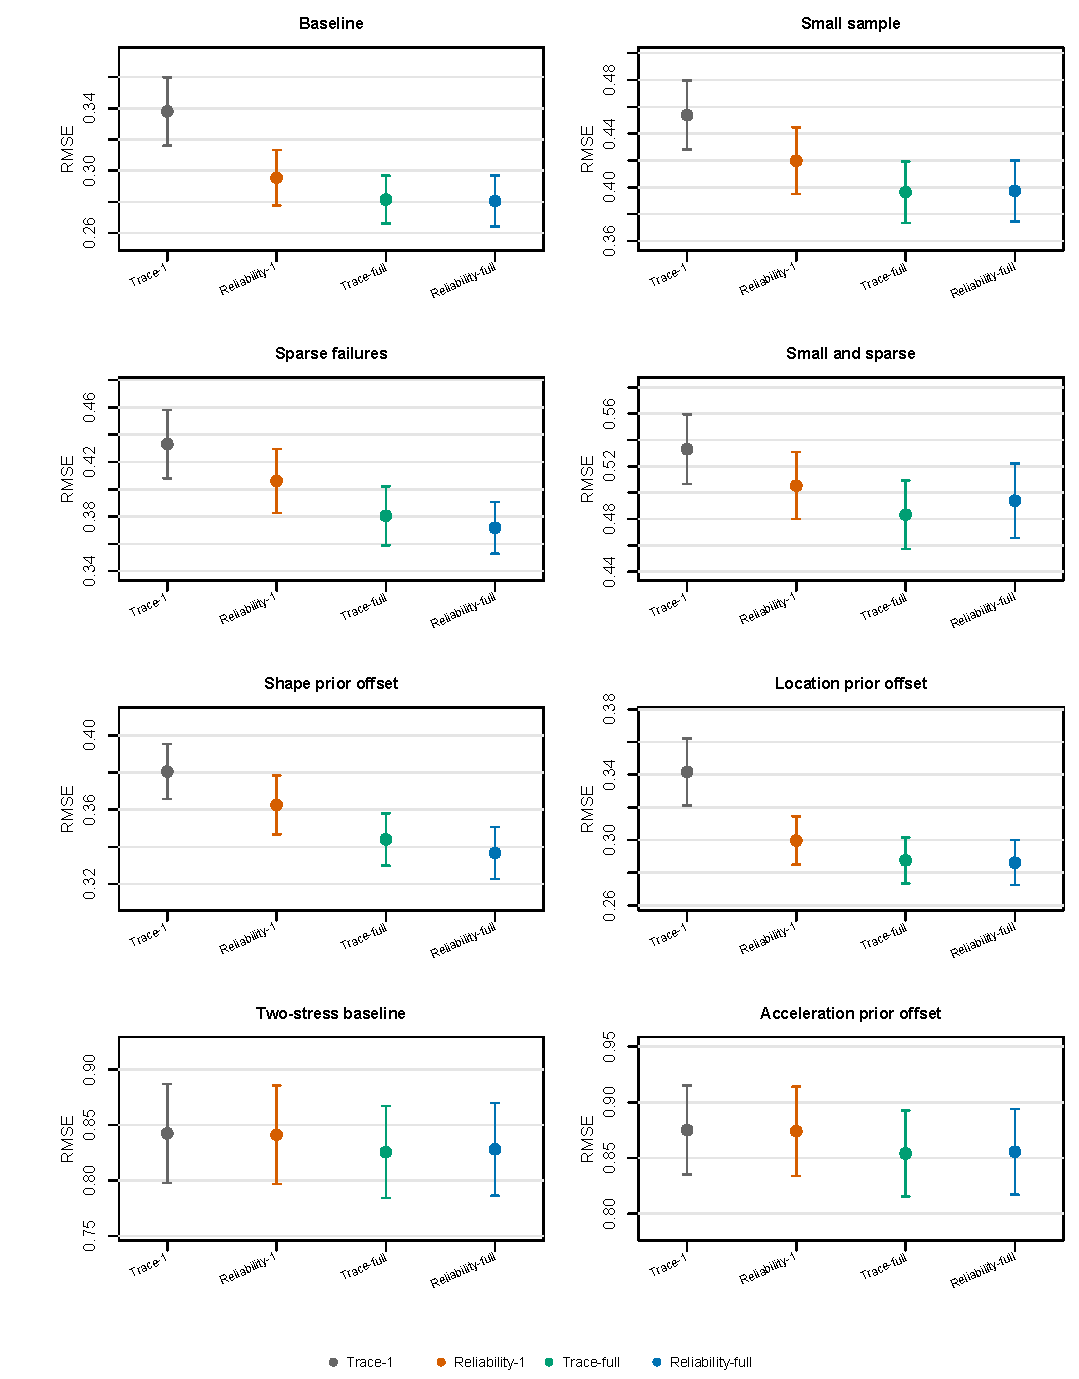
\includegraphics[width=0.95\textwidth]{../output/revision_rmse.pdf}
\caption{RMSE with 95\% Monte Carlo intervals in the eight settings.}
\label{fig:rmse}
\end{figure}

Static Bayesian planning is also competitive. It matches or outperforms Reliability-full in three of the six single-stress settings. Thus the experiments do not establish a general benefit from repeated replanning. They support full-horizon placement as a useful feature and parameterization invariance as a separate property.

Prior-strength checks repeat the baseline and sparse-failure settings with prior standard deviations halved and doubled. Each comparison uses 1000 replicates. Reductions for Reliability-full relative to Reliability-1 range from \PriorReductionMin\% to \PriorReductionMax\%. Under the current prior, the reductions are \PriorCurrentBaselineReduction\% \PriorCurrentBaselineCI\% in the baseline and \PriorCurrentSparseReduction\% \PriorCurrentSparseCI\% for sparse failures. Both weak-prior intervals include zero, while current and diffuse prior intervals lie above zero. The size of the advantage therefore depends on prior concentration (Table \ref{tab:prior}).

\begin{table}[t]
\centering
\caption{Prior-strength sensitivity. Prior SD denotes weak (0.4, 0.4, 0.25), current (0.8, 0.8, 0.5), and diffuse (1.6, 1.6, 1.0) standard deviations for $(\alpha,\beta,\log\sigma)$. Reduction compares Reliability-full with Reliability-1.}
\label{tab:prior}
\resizebox{\textwidth}{!}{% Model version: weibull-cloglog-z0-v2
\begin{tabular}{llrrrrr}
\toprule
Scenario & Prior SD & Fixed & Static & Reliability-1 & Reliability-full & Reduction (\%) \\
\midrule
Baseline & Weak & 0.238 & 0.238 & 0.242 & 0.238 & 1.7 \\
 & Current & 0.282 & 0.283 & 0.295 & 0.281 & 5.1 \\
 & Diffuse & 0.298 & 0.297 & 0.325 & 0.297 & 8.5 \\
\midrule
Sparse failures & Weak & 0.301 & 0.299 & 0.306 & 0.300 & 1.8 \\
 & Current & 0.376 & 0.371 & 0.406 & 0.372 & 8.5 \\
 & Diffuse & 0.413 & 0.408 & 0.491 & 0.406 & 17.4 \\
\bottomrule
\end{tabular}
}
\end{table}

\subsection{Separating posterior averaging from criterion choice}

A second factorial experiment uses two common pilot inspections at 200 and 400 hours so that a point-estimate policy can identify the three joint parameters. It compares plug-in trace, Bayesian trace, plug-in reliability, and Bayesian reliability. All policies use the same final posterior estimator, so the comparison concerns planning decisions. Table \ref{tab:factorial} shows that all four RMSE values are close in each setting.

\begin{table}[t]
\centering
\caption{Factorial comparison over 1000 matched replicates. Entries are RMSE (Monte Carlo standard error).}
\label{tab:factorial}
\resizebox{\textwidth}{!}{% Model version: weibull-cloglog-z0-v2
\begin{tabular}{lrrrr}
\toprule
Scenario & Plug-in trace & Bayesian trace & Plug-in reliability & Bayesian reliability \\
\midrule
Two-stress baseline & 0.825 (0.021) & 0.826 (0.021) & 0.834 (0.021) & 0.826 (0.021) \\
Acceleration prior offset & 0.854 (0.020) & 0.856 (0.020) & 0.868 (0.020) & 0.856 (0.020) \\
\bottomrule
\end{tabular}
}
\end{table}

Bayesian reliability versus Bayesian trace gives an RMSE reduction of -0.03\% in the baseline, with 95\% paired interval $[-0.25,0.18]\%$, and -0.02\% under acceleration-prior offset, with interval $[-0.22,0.17]\%$. Posterior averaging therefore does not provide a separate accuracy advantage in these experiments. Table \ref{tab:factorialreduction} reports the remaining paired contrasts.

\begin{table}[t]
\centering
\caption{Paired RMSE reductions in the factorial experiments. Positive values favor the first policy.}
\label{tab:factorialreduction}
\resizebox{\textwidth}{!}{% Model version: weibull-cloglog-z0-v2
\begin{tabular}{lrrrr}
\toprule
 & \multicolumn{2}{c}{Two-stress baseline} & \multicolumn{2}{c}{Acceleration offset} \\
\cmidrule(lr){2-3} \cmidrule(lr){4-5}
Comparison & Reduction (\%) & 95\% CI & Reduction (\%) & 95\% CI \\
\midrule
Bayesian reliability vs Plug-in trace & -0.191 & [-0.658, 0.207] & -0.189 & [-0.718, 0.246] \\
Bayesian trace vs Plug-in trace & -0.159 & [-0.609, 0.217] & -0.164 & [-0.688, 0.242] \\
Plug-in reliability vs Plug-in trace & -1.148 & [-3.041, 0.605] & -1.649 & [-3.401, -0.003] \\
Bayesian reliability vs Bayesian trace & -0.032 & [-0.245, 0.176] & -0.025 & [-0.217, 0.168] \\
Bayesian reliability vs Plug-in reliability & 0.946 & [-0.757, 2.710] & 1.436 & [-0.316, 3.240] \\
\bottomrule
\end{tabular}
}
\end{table}

Table \ref{tab:computation} summarizes planning time. Across the eight settings, Reliability-full averages 0.546 s per replicate versus 0.426 s for Trace-full, about 28\% more time on average. Reliability-full is faster in the small-sample and small-and-sparse settings and slower in the other six, so the computational difference depends on the scenario.

\begin{table}[t]
\centering
\caption{Mean planning time per replicate in seconds, excluding likelihood fitting.}
\label{tab:computation}
\scriptsize\setlength{\tabcolsep}{2pt}% Model version: weibull-cloglog-z0-v2
\begin{tabular}{lrrrr}
\toprule
Scenario & Trace-1 & Reliability-1 & Trace-full & Reliability-full \\
\midrule
Baseline & 0.031 & 0.113 & 0.317 & 0.475 \\
Small sample & 0.033 & 0.082 & 0.400 & 0.328 \\
Sparse failures & 0.024 & 0.079 & 0.331 & 0.339 \\
Small and sparse & 0.026 & 0.071 & 0.401 & 0.373 \\
Shape prior offset & 0.022 & 0.080 & 0.297 & 0.381 \\
Location prior offset & 0.026 & 0.087 & 0.318 & 0.345 \\
Two-stress baseline & 0.066 & 0.094 & 0.758 & 1.077 \\
Acceleration prior offset & 0.065 & 0.092 & 0.585 & 1.047 \\
\bottomrule
\end{tabular}

\end{table}

An outcome-based two-step policy and a 20-replicate refined feasibility check are reported in Appendix \ref{app:outcome}. They do not show a stable advantage over Reliability-full and do not enter the main accuracy conclusion.

\section{Equivalent parameterization experiments}

\subsection{Experimental construction}

The central comparison uses the two joint settings. For stress scale $c\in\{1,2,10\}$, define
\begin{equation}
x^*=cx,\qquad \beta^*=\beta/c,\qquad x_u^*=cx_u.
\end{equation}
This corresponds to $A=\operatorname{diag}(1,1/c,1)$ in \eqref{eq:transform}. The prior mean and standard deviation of $\beta$ are divided by $c$. Failure times are generated with the same random seeds, so the physical data and reliability target are identical across codings. Each scale and policy uses the same 1000 matched replicates. Trace-full, Weighted-full, and Reliability-full use the same posterior grid and rolling implementation.

Table \ref{tab:identity} checks the objective at fixed candidate times and matched posterior draws. For each draw, the relative difference is $|v_1-v_{10}|/\max(|v_1|,10^{-12})$. Maximum absolute differences are below $3.3\times10^{-6}$ and maximum relative differences are below $7\times10^{-6}$, while mean trace utility changes by nearly an order of magnitude at scale 10. The maximum relative difference for the covariance-weighted trace is \MaxWeightedIdentityRelative. This is a direct numerical check of \eqref{eq:invariance}, not a diagnostic of every optimized plan.

\begin{table}[t]
\centering
\caption{Objective checks under equivalent stress codings.}
\label{tab:identity}
\resizebox{\textwidth}{!}{% Model version: weibull-cloglog-z0-v2
\begin{tabular}{lllrr}
\toprule
Scenario & Max. absolute difference & Max. relative difference & Trace at scale 1 & Trace at scale 10 \\
\midrule
Two-stress baseline & $3.22\times10^{-6}$ & $4.37\times10^{-6}$ & 121.45 & 1072.30 \\
Acceleration prior offset & $3.23\times10^{-6}$ & $5.82\times10^{-6}$ & 73.97 & 651.58 \\
\bottomrule
\end{tabular}
}
\end{table}

\subsection{Inspection schedule changes}

For each replicate and coding comparison, we compute the maximum absolute difference among the five inspection times. Table \ref{tab:schedule} reports its median, 90th percentile, and maximum. At scale 10, median changes for Trace-full are 72.58 h in the baseline and 68.48 h under acceleration-prior offset. The corresponding Reliability-full medians are 0.015 and 0.014 h. Scale 2 produces the same ordering, with Trace-full medians of 8.69 and 9.17 h and Reliability-full medians of 0.009 h.

\begin{table}[t]
\centering
\caption{Maximum inspection-time differences across equivalent codings, in hours.}
\label{tab:schedule}
\resizebox{\textwidth}{!}{% Model version: weibull-cloglog-z0-v2
\begin{tabular}{lllrrr}
\toprule
Scenario & Coding comparison & Policy & Median & 90th percentile & Maximum \\
\midrule
Acceleration prior offset & 1 vs 10 & Reliability-full & 0.01 & 5.69 & 235.32 \\
Two-stress baseline & 1 vs 10 & Reliability-full & 0.01 & 5.65 & 111.46 \\
Acceleration prior offset & 1 vs 10 & Trace-full & 68.48 & 105.29 & 456.91 \\
Two-stress baseline & 1 vs 10 & Trace-full & 72.58 & 108.17 & 303.55 \\
Acceleration prior offset & 1 vs 2 & Reliability-full & 0.01 & 5.96 & 235.35 \\
Two-stress baseline & 1 vs 2 & Reliability-full & 0.01 & 4.35 & 124.36 \\
Acceleration prior offset & 1 vs 2 & Trace-full & 9.17 & 26.63 & 96.68 \\
Two-stress baseline & 1 vs 2 & Trace-full & 8.69 & 25.98 & 136.10 \\
\bottomrule
\end{tabular}
}
\end{table}

For an operational outcome, define the first-detection time as the earliest scheduled inspection at or after the first physical failure, and record its inspection-stage index. Cross-coding comparisons use the same failure times and saved schedules, without reoptimization. We report the absolute time difference and whether the detection stage is unchanged.

\subsection{Common-posterior fixed-pilot verification}
\label{sec:commonposterior}

A separate fixed-pilot experiment verifies the objective transformation and isolates optimization from changes in the rolling observation history. It uses the same pilot data, exactly transformed posteriors, and the same physical posterior draws under codings 1 and 10. Let $\mathcal V_c$ be the full-horizon objective under coding $c$, and let $\hat{\boldsymbol\tau}_c$ be the plan optimized under that coding. Inspection times remain in hours when plans are mapped between codings. Both plans are evaluated in both directions:
\begin{equation}
r_1=\mathcal V_1(\hat{\boldsymbol\tau}_{10})-\mathcal V_1(\hat{\boldsymbol\tau}_1),\qquad
r_{10}=\mathcal V_{10}(\hat{\boldsymbol\tau}_1)-\mathcal V_{10}(\hat{\boldsymbol\tau}_{10}),\qquad
r=\max(|r_1|,|r_{10}|).
\end{equation}
At the respective global optima, $r_1$ and $r_{10}$ are nonnegative; the absolute values accommodate finite optimizer error. Thus $r$ measures excess mean log variance against the optimum found in each coding, rather than a difference between objective sums accumulated along different rolling histories. Because $\mathcal V$ is on the log-variance scale, a difference $d$ corresponds to a multiplicative variance difference of $\exp(d)-1$.

\begin{table}[t]
\centering
\caption{Common-posterior fixed-pilot cross-coding regret over 1000 replicates. The time thresholds refer to this optimization experiment, not to the rolling schedules in Table \ref{tab:schedule}.}
\label{tab:regret}
\resizebox{\textwidth}{!}{% Model version: weibull-cloglog-z0-v2
\begin{tabular}{lllrrrrr}
\toprule
Scenario & Comparison & Policy & Median regret & 90th regret & $>1$ h (\%) & $>5$ h (\%) & $>10$ h (\%) \\
\midrule
Two-stress baseline & 1 vs 10 & Reliability-full & $8.33\times10^{-16}$ & $5.20\times10^{-14}$ & 0.0 & 0.0 & 0.0 \\
Acceleration prior offset & 1 vs 10 & Reliability-full & $1.11\times10^{-15}$ & $4.11\times10^{-14}$ & 0.0 & 0.0 & 0.0 \\
\bottomrule
\end{tabular}
}
\end{table}

Median and 90th-percentile bidirectional regrets are numerically negligible in both scenarios under the main settings; the exact values in Table \ref{tab:regret} are retained for reproducibility. These checks verify the common-input implementation and do not replace the rolling schedule diagnostics.

Figure \ref{fig:codings} shows baseline replicate 1, generated with seed 71001 and selected before inspecting the schedules. Trace-full changes its second inspection appreciably across codings, whereas the Reliability-full points nearly overlap.

\begin{figure}[pos=t]
\centering
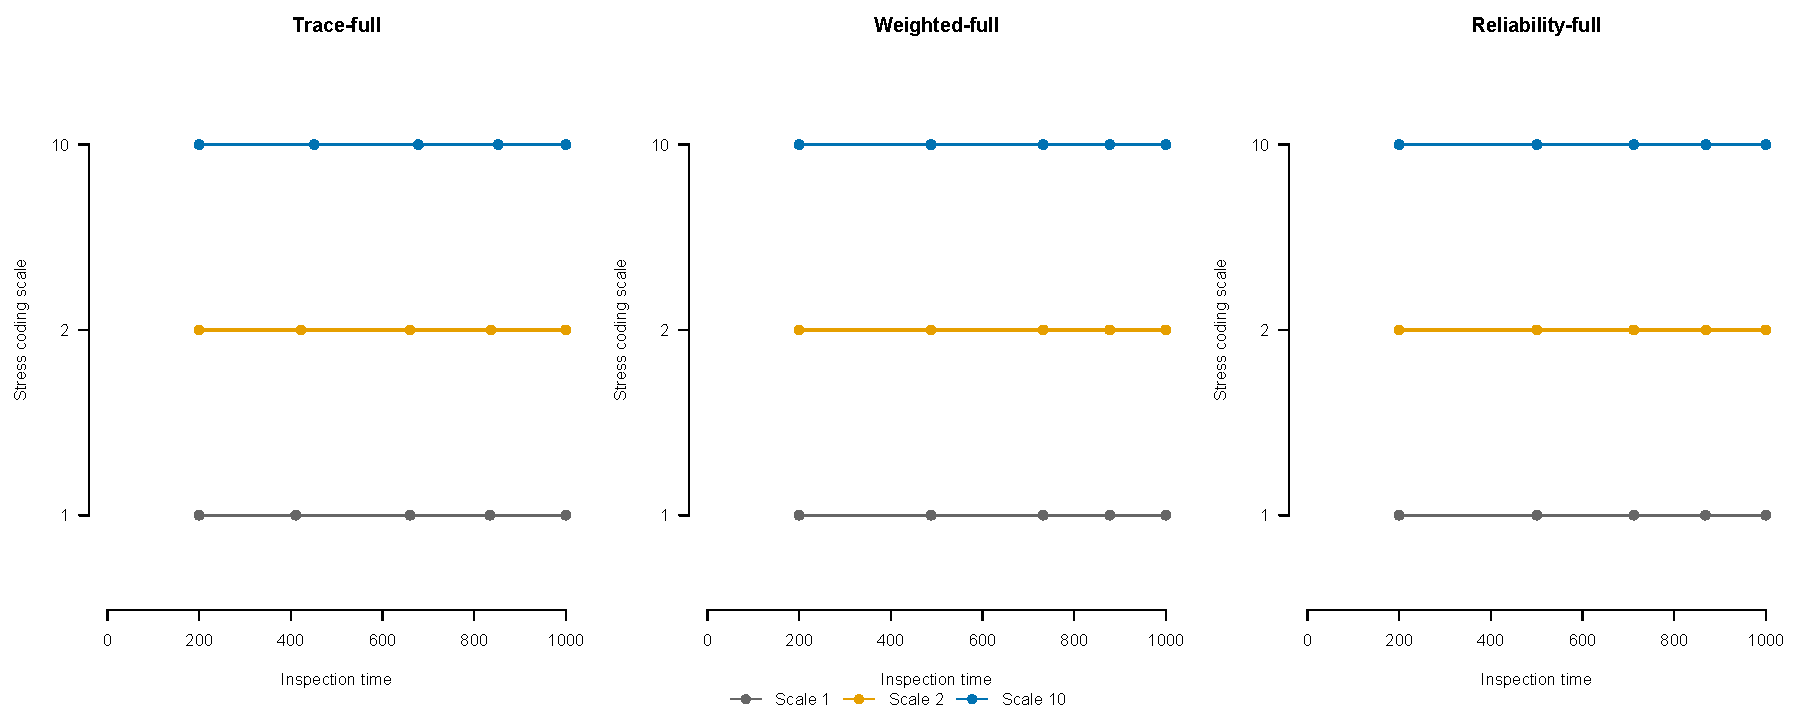
\includegraphics[width=\textwidth]{../output/parameterization_schedules.pdf}
\caption{Inspection schedules for one baseline replicate under three equivalent stress codings.}
\label{fig:codings}
\end{figure}

\subsection{Accuracy across codings}

Table \ref{tab:codingaccuracy} shows that the coding comparison does not trade invariance for a material change in accuracy. Trace-full RMSE varies by less than 0.003 across scales, and Reliability-full RMSE varies by less than 0.001. This supports a limited conclusion: Reliability-full preserves the design objective across equivalent codings while maintaining comparable accuracy. It does not imply better estimation or identical numerical schedules in every replicate.

\begin{table}[t]
\centering
\caption{RMSE (Monte Carlo standard error) under equivalent stress codings.}
\label{tab:codingaccuracy}
\resizebox{\textwidth}{!}{% Model version: weibull-cloglog-z0-v2
\begin{tabular}{llrrr}
\toprule
Scenario & Policy & Scale 1 & Scale 2 & Scale 10 \\
\midrule
Two-stress baseline & Trace-full & 0.825 (0.021) & 0.826 (0.021) & 0.828 (0.021) \\
Two-stress baseline & Reliability-full & 0.828 (0.021) & 0.828 (0.021) & 0.828 (0.021) \\
Acceleration prior offset & Trace-full & 0.854 (0.020) & 0.854 (0.020) & 0.856 (0.020) \\
Acceleration prior offset & Reliability-full & 0.856 (0.020) & 0.855 (0.020) & 0.855 (0.020) \\
\bottomrule
\end{tabular}
}
\end{table}

Table \ref{tab:codingreduction} reports the corresponding paired comparisons. Every 95\% interval includes zero, so the coding comparisons show no detectable change in RMSE.

\begin{table}[t]
\centering
\caption{Paired RMSE reductions across equivalent codings. Positive values indicate lower RMSE at the larger scale.}
\label{tab:codingreduction}
\scriptsize\setlength{\tabcolsep}{2pt}% Model version: weibull-cloglog-z0-v2
\begin{tabular}{lllrr}
\toprule
Scenario & Policy & Comparison & Reduction (\%) & 95\% paired CI \\
\midrule
Two-stress baseline & Trace-full & 2 vs 1 & 0.00 & [-0.13, 0.13] \\
Two-stress baseline & Trace-full & 10 vs 1 & -0.33 & [-0.71, 0.06] \\
Two-stress baseline & Reliability-full & 2 vs 1 & 0.01 & [-0.06, 0.08] \\
Two-stress baseline & Reliability-full & 10 vs 1 & 0.05 & [-0.02, 0.12] \\
Acceleration prior offset & Trace-full & 2 vs 1 & 0.02 & [-0.16, 0.21] \\
Acceleration prior offset & Trace-full & 10 vs 1 & -0.24 & [-0.65, 0.14] \\
Acceleration prior offset & Reliability-full & 2 vs 1 & 0.04 & [-0.03, 0.13] \\
Acceleration prior offset & Reliability-full & 10 vs 1 & 0.05 & [-0.01, 0.13] \\
\bottomrule
\end{tabular}

\end{table}

\subsection{Weighted trace and first-detection outcomes}

Table \ref{tab:weightedtrace} compares the invariant alternatives with the unweighted trace. Weighted-full has median schedule differences of 0.009 h in both settings, with 90th percentiles of 8.39 and 9.87 h. Reliability-full has medians of 0.015 and 0.014 h and 90th percentiles of 5.65 and 5.69 h. The RMSE values are close for all three policies. Weighted-full therefore provides another invariant choice; the reliability criterion is distinguished by directly targeting use-stress reliability, not by unique invariance.

The first-detection stage is unchanged in all 1000 matched pairs for every policy. Nevertheless, the unweighted trace gives first-detection time differences above 1 h in 7.3\% and 7.4\% of pairs, compared with none for Weighted-full or Reliability-full. Coding sensitivity therefore affects the reproducibility of inspection and detection timing rather than the ordering of the first detection.

The common pilot had already revealed a failure in 927 baseline pairs and 925 prior-offset pairs. Among the remaining 73 and 75 pairs, median cross-coding detection-time differences for Trace-full were 25.95 and 31.35 h, and 100\% and 98.7\% exceeded 1 h. Neither invariant criterion had such a difference. Every pair had a detected failure by its last inspection, so no pair required an undetected-case adjustment.

\begin{table}[t]
\centering
\caption{Weighted-trace and operational comparisons between stress scales 1 and 10. Schedule $\Delta t$ is the maximum absolute difference among inspection times. Detection $\Delta t$ is the absolute difference in first-detection time. The detection-stage index is unchanged in all matched pairs.}
\label{tab:weightedtrace}
\resizebox{\textwidth}{!}{% Model version: weibull-cloglog-z0-v2
\begin{tabular}{llrrrrrr}
\toprule
Scenario & Policy & Median $\Delta t$ & 90th $\Delta t$ & RMSE (scale 1) & RMSE (scale 10) & $>1$ h detection (\%) & Max. detection $\Delta t$ \\
\midrule
Two-stress baseline & Trace-full & 72.58 & 108.17 & 0.825 & 0.828 & 7.3 & 186.713 \\
Two-stress baseline & Weighted-full & 0.01 & 8.39 & 0.828 & 0.828 & 0.0 & 0.025 \\
Two-stress baseline & Reliability-full & 0.01 & 5.65 & 0.828 & 0.828 & 0.0 & 0.095 \\
Acceleration prior offset & Trace-full & 68.48 & 105.29 & 0.854 & 0.856 & 7.4 & 171.392 \\
Acceleration prior offset & Weighted-full & 0.01 & 9.87 & 0.857 & 0.857 & 0.0 & 0.901 \\
Acceleration prior offset & Reliability-full & 0.01 & 5.69 & 0.856 & 0.855 & 0.0 & 0.097 \\
\bottomrule
\end{tabular}
}
\end{table}

Additional checks vary posterior grids, posterior draws, and optimization starts. Additional starts changed some nearly equivalent plans but did not consistently reduce schedule or regret quantiles. Rolling sensitivity remained, whereas common-posterior checks showed numerically negligible bidirectional regret. The diagnostic tables use the first 200 replicates and are not directly comparable with the full-sample RMSE values above. Full results are given in Appendix \ref{app:numerical}.

\section{Voltage ALT illustration}
\label{sec:voltage}

We illustrate the workflow using 24 capacitor failure times at 80, 100, and 120 V, with eight units per voltage \citep{yang2007}. A Weibull inverse-power model is used. The 80 and 100 V groups provide historical information, while the 120 V group is treated as a new interval-monitored group. The target is $R(1000)$ at 60 V. The normalized coordinate is $x=\{\log(V)-\log(120)\}/\log(120/80)$. The alternative coordinate $\log(V/120)$ multiplies $x$ by $\log(120/80)$ and transforms the acceleration coefficient and its prior accordingly.

Historical fitting is used only to construct the empirical prior. The new-data posterior is
\begin{equation}
p(\theta\mid D_{\mathrm{new}})\propto
\pi_{\mathrm{emp}}(\theta\mid D_{\mathrm{hist}})L_{\mathrm{new}}(\theta),
\end{equation}
so the historical likelihood does not appear again. The new group has a common pilot at 500 h, five inspections, and a latest permissible time of 2500 h. Trace-full, Weighted-full, and Reliability-full use 40 planning draws and 30 additional starts. Survivors are right-censored at the actual last inspection.

Table \ref{tab:voltage} shows the resulting schedules and target estimates. The two codings produce identical interval counts. Maximum schedule differences are 0.080, 0.042, and below 0.001 h for Trace-full, Weighted-full, and Reliability-full, respectively. Reliability-full reveals the first failure at 899.8 h, compared with 1303.6 and 1413.4 h for the trace policies. This is a descriptive result for one retrospective dataset, not evidence of a general detection-time advantage.

\begin{table}[t]
\centering
\caption{Voltage ALT plans. The target is $h=\log\{-\log R(1000)\}$ at 60 V. Schedules are shown for the normalized coding. Max. schedule $\Delta t$ compares the normalized and log-ratio codings. No failure had occurred at the 500 h pilot.}
\label{tab:voltage}
\resizebox{\textwidth}{!}{% Model version: weibull-cloglog-z0-v2
\begin{tabular}{llrrrr}
\toprule
Policy & Inspection times (h) & $h$ (normalized) & $h$ (log ratio) & Max. schedule $\Delta t$ & First detection (h) \\
\midrule
Trace-full & 500.000, 1303.589, 1555.061, 1820.016, 2288.217 & -4.790 & -4.790 & 0.080 & 1303.6 \\
Weighted-full & 500.000, 1413.418, 1642.128, 1979.510, 2500.000 & -4.350 & -4.350 & 0.042 & 1413.4 \\
Reliability-full & 500.000, 899.765, 1254.530, 1844.908, 2499.999 & -5.030 & -5.030 & 0.000 & 899.8 \\
\bottomrule
\end{tabular}
}
\end{table}

A parametric bootstrap anchored to the fit to all 24 observations gives 200 matched replicates. Normalized-coordinate RMSE values are 3.907, 3.950, and 3.934 for Trace-full, Weighted-full, and Reliability-full; the log-ratio values are 3.907, 3.950, and 3.934 to three decimals. All 90\% posterior intervals contain the anchor target, reflecting wide intervals rather than evidence of sharp prediction. No convergence failures or undetected pairs occur. Eight-fold leave-one-out analysis of the 120 V group gives mean log predictive scores of -7.799, -7.905, and -7.797, respectively. These checks support implementation and numerical consistency, not an accuracy advantage.

\section{Discussion}

The results separate two properties that are easy to conflate in sequential design: estimation accuracy and consistency under reparameterization. Reliability planning does not outperform full-horizon trace planning in the experiments. It does preserve the scalar-target objective when the stress coding and model parameters are transformed together. For applications in which analysts may use different but equivalent stress codings, this property has practical value independent of RMSE rankings.

Unweighted Fisher trace is interpretable when parameter scales are fixed by the scientific problem, but it is not the only possible trace criterion. Weighted-full uses current posterior covariance to obtain an invariant alternative with comparable accuracy. Its small median schedule differences and larger upper-tail differences show why objective invariance and numerical plan stability must be reported separately. The reliability criterion offers a direct alternative when reliability at a stated use condition is the primary target; it is not the only invariant choice or a replacement for every RITO application.

The computational results also limit the conclusion. Reliability-full uses about 28\% more planning time than Trace-full on average, with faster planning in two settings and slower planning in six. Posterior grid resolution affects target variance. Objective invariance does not ensure a unique optimizer or identical numerical schedules in the presence of flat directions and local solutions. The reported upper quantiles and outliers are therefore part of the evidence. Additional optimization starts are examined in the numerical diagnostics rather than assumed to remove these discrepancies.

The numerical study assumes a correctly specified Weibull model. Joint settings use a common schedule across stress groups rather than independent asynchronous schedules. The point-estimate trace comparison captures RITO's full-horizon criterion and parameter updating but does not reproduce every feature of the original algorithm. Static Bayesian planning remains competitive in several single-stress settings, and the outcome-lookahead conclusion is limited to the tested two-step approximation. The voltage analysis is retrospective and uses only eight units in the new group.

Future work can examine lifetime-model uncertainty and asynchronous inspection across stress groups. These extensions address different statistical questions and should not be conflated with the invariance result established here.

\section{Conclusions}

This paper embeds a Bayesian scalar-target reliability criterion in RITO-style sequential inspection. Its objective is invariant under invertible linear reparameterization, unlike the unweighted Fisher trace used by RITO. Across eight settings, accuracy is comparable to Trace-full. Equivalent codings materially change trace schedules; common-posterior checks confirm invariance up to numerical precision, while rolling experiments retain numerical sensitivity. The covariance-weighted trace comparator is also invariant, whereas the reliability criterion directly targets the use-stress estimand. The proposed criterion is useful when consistent, reliability-oriented decisions are required, with scenario-dependent computational costs.

\clearpage
\appendix
\section{Additional single-stress comparisons}

Table \ref{tab:fullsingle} gives the full comparison. Fixed is equally spaced, Static optimizes after the pilot without replanning, and Reliability-2 plans two inspections at a time.

\begin{table}[pos=H]
\centering
\caption{Complete single-stress RMSE and Monte Carlo standard errors over 1000 matched replicates.}
\label{tab:fullsingle}
\resizebox{\textwidth}{!}{% Model version: weibull-cloglog-z0-v2
\begin{tabular}{lrrrrrr}
\toprule
Scenario & Fixed & Static & Reliability-1 & Reliability-2 & Reliability-full & Outcome-2 \\
\midrule
Baseline & 0.282 (0.008) & 0.283 (0.008) & 0.295 (0.009) & 0.284 (0.009) & 0.281 (0.008) & 0.280 (0.008) \\
Small sample & 0.398 (0.013) & 0.397 (0.011) & 0.420 (0.013) & 0.400 (0.012) & 0.397 (0.012) & 0.399 (0.012) \\
Sparse failures & 0.376 (0.010) & 0.371 (0.010) & 0.406 (0.012) & 0.379 (0.011) & 0.372 (0.010) & 0.380 (0.011) \\
Small and sparse & 0.486 (0.013) & 0.492 (0.015) & 0.505 (0.013) & 0.496 (0.014) & 0.494 (0.014) & 0.484 (0.013) \\
Shape prior offset & 0.341 (0.007) & 0.339 (0.007) & 0.363 (0.008) & 0.344 (0.007) & 0.337 (0.007) & 0.350 (0.007) \\
Location prior offset & 0.287 (0.007) & 0.290 (0.007) & 0.300 (0.008) & 0.289 (0.007) & 0.286 (0.007) & 0.293 (0.007) \\
\bottomrule
\end{tabular}
}
\end{table}

\begin{table}[pos=H]
\centering
\caption{Paired RMSE reductions and 95\% bootstrap intervals. Positive values favor the first policy.}
\label{tab:singlereductions}
\resizebox{\textwidth}{!}{% Model version: weibull-cloglog-z0-v2
\begin{tabular}{lrrrr}
\toprule
Scenario & \multicolumn{2}{c}{Reliability-full vs Reliability-1} & \multicolumn{2}{c}{Outcome-2 vs Reliability-full} \\
\cmidrule(lr){2-3} \cmidrule(lr){4-5}
 & Reduction (\%) & 95\% CI & Reduction (\%) & 95\% CI \\
\midrule
Baseline & 5.06 & [2.15, 8.14] & 0.18 & [-1.68, 2.05] \\
Small sample & 5.36 & [2.62, 8.10] & -0.44 & [-2.24, 1.30] \\
Sparse failures & 8.48 & [5.73, 11.24] & -2.16 & [-4.14, -0.18] \\
Small and sparse & 2.26 & [-1.54, 5.94] & 2.08 & [0.04, 4.14] \\
Shape prior offset & 7.14 & [4.39, 9.99] & -3.85 & [-5.59, -2.11] \\
Location prior offset & 4.51 & [2.15, 6.84] & -2.40 & [-4.23, -0.63] \\
\bottomrule
\end{tabular}
}
\end{table}

\clearpage
\section{Numerical and optimizer diagnostics}
\label{app:numerical}

\subsection{Grid and optimizer checks for pilot datasets}

\begin{table}[pos=H]
\centering
\caption{Grid and optimizer checks for pilot replicate 1. Multi-start adds four random starts to the default start. Every plan is evaluated on the finest-grid posterior for that scenario using the same 256 draws. Regret is the excess mean log variance relative to the best value found among the evaluated plans, and $\Delta t_{\mathrm{MS}}$ is the maximum time difference between default and multi-start plans.}
\label{tab:grid}
\resizebox{\textwidth}{!}{% Model version: weibull-cloglog-z0-v2
\begin{tabular}{llrlrrr}
\toprule
Scenario & Grid & Variance & Default plan & Default regret & Multi-start regret & $\Delta t_{\mathrm{MS}}$ \\
\midrule
Baseline & 41 & 0.339 & 289.1;393.21;514.49;662.73 & $5.93\times10^{-5}$ & $1.34\times10^{-7}$ & 337.24 \\
Baseline & 61 & 0.333 & 290.1;395.69;518.89;668.89 & $6.13\times10^{-5}$ & $1.03\times10^{-6}$ & 331.08 \\
Baseline & 101 & 0.336 & 329.21;489.11;695.48;999.97 & $0$ & $0$ & 0.00 \\
\midrule
Two-stress baseline & 21 & 4.775 & 507.31;666.82;815.91;1000 & $8.13\times10^{-5}$ & $8.13\times10^{-5}$ & 0.00 \\
Two-stress baseline & 31 & 4.882 & 429.86;640.15;814.57;1000 & $1.80\times10^{-4}$ & $1.80\times10^{-4}$ & 0.00 \\
Two-stress baseline & 41 & 5.002 & 490.29;674.35;829.82;1000 & $7.52\times10^{-12}$ & $0$ & 0.01 \\
Acceleration prior offset & 21 & 2.011 & 425.8;577.69;772.05;1000 & $1.93\times10^{-4}$ & $1.93\times10^{-4}$ & 0.00 \\
Acceleration prior offset & 31 & 1.984 & 446.71;622.5;799.54;1000 & $3.91\times10^{-5}$ & $3.91\times10^{-5}$ & 0.00 \\
Acceleration prior offset & 41 & 1.961 & 437.59;610.54;784.32;1000 & $3.09\times10^{-10}$ & $0$ & 0.03 \\
\bottomrule
\end{tabular}
}
\end{table}

The single-stress default plans at grid sizes 41 and 61 end near 663 and 669 h, whereas their multi-start plans end near 1000 h. Despite differences of 337.24 and 331.08 h, their default regrets are only $5.93\times10^{-5}$ and $6.13\times10^{-5}$. Multi-start optimization reduces these values to $1.34\times10^{-7}$ and $1.03\times10^{-6}$. The joint cases show a different pattern: additional starts change the default plans by at most 0.03 h and do not remove the differences between grid-specific plans. Their default regrets on the common reference objectives are at most $1.94\times10^{-4}$. Posterior variance alone is therefore not a sufficient measure of planning stability, and large time differences can accompany nearly equivalent objective values.

\subsection{Rolling numerical sensitivity}

Additional checks use the first 200 replicates to compare 16, 32, and 64 posterior draws and grid resolutions of 21, 31, and 41 points per direction. All rows concern Reliability-full. Posterior-draw checks fix the grid at 21 points per direction, and grid checks use 16 draws. The same seeds are used across settings, but different grids do not produce identical continuous posterior draws. Table \ref{tab:sensitivity} therefore describes the combined rolling effects of posterior discretization, sampling, and optimization rather than a pure optimizer comparison. The scale-1 RMSE values at the main setting exactly reproduce the first 200 rows of the main simulations. For reference, the corresponding full-sample values in Table \ref{tab:codingaccuracy} are 0.825 and 0.856; the diagnostic subsample values should not be compared directly with them.

\begin{table}[pos=H]
\centering
\caption{Rolling numerical sensitivity over the first 200 replicates. Extra starts are added to the equally spaced and available warm starts; four extra starts are examined at grid size 41. $\Delta t$ is the maximum inspection-time difference between scale 1 and scale 10. Seconds include only the planning optimizer and exclude posterior grid construction and final estimation. RMSE values are based on the first 200 replicates and are not directly comparable with the full-sample values in Table \ref{tab:codingaccuracy}.}
\label{tab:sensitivity}
\resizebox{\textwidth}{!}{% Model version: weibull-cloglog-z0-v2
\begin{tabular}{lllrrrrrr}
\toprule
Scenario & Setting & Value & Extra starts & Median $\Delta t$ & 90th $\Delta t$ & RMSE (scale 1) & RMSE (scale 10) & Seconds \\
\midrule
Two-stress baseline & Posterior draws & 16 & 0 & 0.02 & 4.92 & 0.705 & 0.705 & 1.045 \\
Two-stress baseline & Posterior draws & 32 & 0 & 0.03 & 5.96 & 0.706 & 0.707 & 2.073 \\
Two-stress baseline & Posterior draws & 64 & 0 & 0.32 & 6.43 & 0.704 & 0.704 & 4.135 \\
Acceleration prior offset & Posterior draws & 16 & 0 & 0.01 & 5.69 & 0.861 & 0.860 & 1.031 \\
Acceleration prior offset & Posterior draws & 32 & 0 & 0.03 & 5.50 & 0.861 & 0.862 & 2.045 \\
Acceleration prior offset & Posterior draws & 64 & 0 & 0.08 & 5.14 & 0.861 & 0.861 & 4.064 \\
Two-stress baseline & Grid points & 21 & 0 & 0.02 & 4.92 & 0.705 & 0.705 & 1.041 \\
Two-stress baseline & Grid points & 31 & 0 & 0.34 & 12.82 & 0.703 & 0.704 & 1.039 \\
Two-stress baseline & Grid points & 41 & 0 & 0.43 & 15.28 & 0.709 & 0.712 & 1.044 \\
Two-stress baseline & Grid points & 41 & 4 & 0.52 & 15.43 & 0.710 & 0.712 & 5.590 \\
Acceleration prior offset & Grid points & 21 & 0 & 0.01 & 5.69 & 0.861 & 0.860 & 1.143 \\
Acceleration prior offset & Grid points & 31 & 0 & 0.27 & 11.53 & 0.856 & 0.856 & 1.120 \\
Acceleration prior offset & Grid points & 41 & 0 & 1.34 & 19.63 & 0.857 & 0.857 & 1.044 \\
Acceleration prior offset & Grid points & 41 & 4 & 0.96 & 20.01 & 0.857 & 0.857 & 4.881 \\
\bottomrule
\end{tabular}
}
\end{table}

In the two-stress baseline, four extra starts do not reduce the median or 90th-percentile cross-coding time difference at grid size 41. The two RMSE values change by less than 0.001, while mean planning time increases. Under acceleration-prior offset, additional starts reduce the median difference but increase the 90th percentile and maximum. Thus the effect of additional starts is mixed across scenarios and summary measures, and it does not remove the rolling numerical sensitivity.

\subsection{Common-posterior optimization sensitivity}

Table \ref{tab:commonsensitivity} repeats these settings in the fixed-pilot construction. It also compares the default start with four additional random starts at the main setting and the finest grid. This comparison separates cross-coding optimizer regret from the rolling trajectory differences in Table \ref{tab:sensitivity}.

\begin{table}[pos=H]
\centering
\caption{Common-posterior optimization sensitivity. Regret is the bidirectional excess mean log variance defined in Section \ref{sec:commonposterior}. One start is the default and five starts include four additional random starts. Time differences below 0.001 h are numerically negligible and do not imply exact algebraic equality of all optimized inspection times.}
\label{tab:commonsensitivity}
\resizebox{\textwidth}{!}{% Model version: weibull-cloglog-z0-v2
\begin{tabular}{llrrrrrr}
\toprule
Scenario & Fixed setting & Starts & Replicates & Median $\Delta t$ & 90th $\Delta t$ & Median regret & 90th regret \\
\midrule
Two-stress baseline & Grid 21, draws 16 & 1 & 200 & $<0.001$ & $<0.001$ & $8.33\times10^{-16}$ & $5.44\times10^{-14}$ \\
Two-stress baseline & Grid 21, draws 16 & 5 & 200 & $<0.001$ & $<0.001$ & $4.09\times10^{-16}$ & $4.64\times10^{-13}$ \\
Two-stress baseline & Grid 31, draws 16 & 1 & 200 & $<0.001$ & $<0.001$ & $8.88\times10^{-16}$ & $7.33\times10^{-14}$ \\
Two-stress baseline & Grid 41, draws 16 & 1 & 200 & $<0.001$ & $<0.001$ & $6.38\times10^{-16}$ & $3.76\times10^{-14}$ \\
Two-stress baseline & Grid 41, draws 16 & 5 & 200 & $<0.001$ & $<0.001$ & $4.44\times10^{-16}$ & $6.85\times10^{-13}$ \\
Two-stress baseline & Grid 21, draws 32 & 1 & 200 & $<0.001$ & $<0.001$ & $1.26\times10^{-15}$ & $8.35\times10^{-14}$ \\
Two-stress baseline & Grid 21, draws 64 & 1 & 200 & $<0.001$ & $<0.001$ & $1.14\times10^{-15}$ & $3.57\times10^{-14}$ \\
Acceleration prior offset & Grid 21, draws 16 & 1 & 200 & $<0.001$ & $<0.001$ & $1.11\times10^{-15}$ & $3.71\times10^{-14}$ \\
Acceleration prior offset & Grid 21, draws 16 & 5 & 200 & $<0.001$ & $<0.001$ & $8.57\times10^{-16}$ & $1.20\times10^{-13}$ \\
Acceleration prior offset & Grid 31, draws 16 & 1 & 200 & $<0.001$ & $<0.001$ & $8.92\times10^{-16}$ & $6.66\times10^{-14}$ \\
Acceleration prior offset & Grid 41, draws 16 & 1 & 200 & $<0.001$ & $<0.001$ & $8.88\times10^{-16}$ & $5.88\times10^{-14}$ \\
Acceleration prior offset & Grid 41, draws 16 & 5 & 200 & $<0.001$ & $<0.001$ & $5.07\times10^{-16}$ & $2.28\times10^{-13}$ \\
Acceleration prior offset & Grid 21, draws 32 & 1 & 200 & $<0.001$ & $<0.001$ & $1.11\times10^{-15}$ & $4.16\times10^{-14}$ \\
Acceleration prior offset & Grid 21, draws 64 & 1 & 200 & $<0.001$ & $<0.001$ & $1.10\times10^{-15}$ & $3.65\times10^{-14}$ \\
\bottomrule
\end{tabular}
}
\end{table}

The rolling and fixed-pilot comparisons answer different questions. The former includes changes in posterior approximation and subsequent observations; the latter holds those inputs fixed. Additional starts can select a different nearly equivalent plan and need not reduce every schedule or regret quantile. They are used here as a diagnostic rather than as a guaranteed improvement over the default optimizer. The number of nonfatal optimizer warnings retained in the rolling multi-start analyses is \MultiStartOptimizerWarnings, and their larger planning times are included in Table \ref{tab:sensitivity}.

\section{Outcome-based lookahead}
\label{app:outcome}

A separate two-step policy propagates possible failure counts and optimizes the next inspection conditional on each first-stage outcome. Outcome-2 gives slightly lower RMSE in the baseline and small-and-sparse settings and higher RMSE in the other four settings, with no stable advantage over Reliability-full. A refined version uses 12 candidate times, seven outcome nodes, and 20 posterior draws. Over 20 baseline replicates, its RMSE is \HighResolutionOutcomeRMSE, compared with \HighResolutionBatchRMSE{} for Reliability-full, and mean planning time is \HighResolutionOutcomeTime{} s. This feasibility check shows no material difference and is not used to judge outcome-based design more generally.

\section*{Declarations}

\subsection*{Funding}
This work was supported by the Jiangsu Provincial Natural Science Foundation for Young Scholars.

\subsection*{Competing interests}
The authors declare no competing interests.

\subsection*{Data and code availability}
The R code and saved outputs used in this study are provided as supplementary material. The full entry point is `run\_all.R`; after the simulations are complete, `rebuild\_manuscript.R` regenerates all manuscript objects without repeating them. Numerical diagnostics select the first 200 replicates using `replicate <= 200`. A full serial rerun takes several hours; rebuilding from the saved outputs takes about one minute. Model checks are in `validate\_model.R`, and output checks are in `validate\_results.R`, `validate\_second\_round.R`, and `validate\_manuscript.R`. Random seeds, raw outputs, model-version identifiers, and session information are included. The code corresponds to the revised manuscript with reliability target $h=z_0$.

\subsection*{Author contributions}
Wenhan Zhang: conceptualization, methodology, software, formal analysis, investigation, writing, and visualization. Xiaojun Zhu: conceptualization, supervision, and writing review and editing.

\bibliographystyle{elsarticle-num}
\bibliography{references}

\end{document}
